\documentclass[aspectratio=169]{../latex_main/tntbeamer}  % you can pass all options of the beamer class, e.g., 'handout' or 'aspectratio=43'
\usepackage{dsfont}
\usepackage{bm}
\usepackage[english]{babel}
\usepackage[T1]{fontenc}
%\usepackage[utf8]{inputenc}
\usepackage{graphicx}
\graphicspath{ {./figures/} }
\usepackage{algorithm}
\usepackage[ruled,vlined,algo2e,linesnumbered]{algorithm2e}
\usepackage{hyperref}
\usepackage{booktabs}
\usepackage{mathtools}

\usepackage{amsmath,amssymb}

\DeclareMathOperator*{\argmax}{arg\,max}
\DeclareMathOperator*{\argmin}{arg\,min}

\usepackage{amsbsy}
\newcommand{\vect}[1]{\bm{#1}}
%\newcommand{\vect}[1]{\boldsymbol{#1}}

\usepackage{pgfplots}
\pgfplotsset{compat=1.16}
\usepackage{tikz}
\usetikzlibrary{trees} 
\usetikzlibrary{shapes.geometric}
\usetikzlibrary{positioning,shapes,shadows,arrows,calc,mindmap}
\usetikzlibrary{positioning,fadings,through}
\usetikzlibrary{decorations.pathreplacing}
\usetikzlibrary{intersections}
\pgfdeclarelayer{background}
\pgfdeclarelayer{foreground}
\pgfsetlayers{background,main,foreground}
\tikzstyle{activity}=[rectangle, draw=black, rounded corners, text centered, text width=8em]
\tikzstyle{data}=[rectangle, draw=black, text centered, text width=8em]
\tikzstyle{myarrow}=[->, thick, draw=black]

% Define the layers to draw the diagram
\pgfdeclarelayer{background}
\pgfdeclarelayer{foreground}
\pgfsetlayers{background,main,foreground}

% Requires XeLaTeX or LuaLaTeX
%\usepackage{unicode-math}

\usepackage{fontspec}
%\setsansfont{Arial}
\setsansfont{RotisSansSerifStd}[ 
Path=../latex_main/fonts/,
Extension = .otf,
UprightFont = *-Regular,  % or *-Light
BoldFont = *-ExtraBold,  % or *-Bold
ItalicFont = *-Italic
]
\setmonofont{Cascadia Mono}[
Scale=0.8
]

% scale factor adapted; mathrm font added (Benjamin Spitschan @TNT, 2021-06-01)
%\setmathfont[Scale=1.05]{Libertinus Math}
%\setmathrm[Scale=1.05]{Libertinus Math}

% other available math fonts are (not exhaustive)
% Latin Modern Math
% XITS Math
% Libertinus Math
% Asana Math
% Fira Math
% TeX Gyre Pagella Math
% TeX Gyre Bonum Math
% TeX Gyre Schola Math
% TeX Gyre Termes Math

% Literature References
\newcommand{\lit}[2]{\href{#2}{\footnotesize\color{black!60}[#1]}}

%%% Beamer Customization
%----------------------------------------------------------------------
% (Don't) Show sections in frame header. Options: 'sections', 'sections light', empty
\setbeamertemplate{headline}{empty}

% Add header logo for normal frames
\setheaderimage{
	% 
\includegraphics[height=\logoheight]{figures/TNT_darkv4.pdf}
	
\includegraphics[height=\logoheight]{../latex_main/figures/luh_logo_rgb_0_80_155.pdf}
	% 
\includegraphics[height=\logoheight]{figures/logo_tntluh.pdf}
}

% Header logo for title page
\settitleheaderimage{
	% 
\includegraphics[height=\logoheight]{figures/TNT_darkv4.pdf}
	
\includegraphics[height=\logoheight]{../latex_main/figures/luh_logo_rgb_0_80_155.pdf}
	% 
\includegraphics[height=\logoheight]{figures/logo_tntluh.pdf}
}

% Title page: tntdefault 
\setbeamertemplate{title page}[tntdefault]  % or luhstyle
% Add optional title image here
%\addtitlepageimagedefault{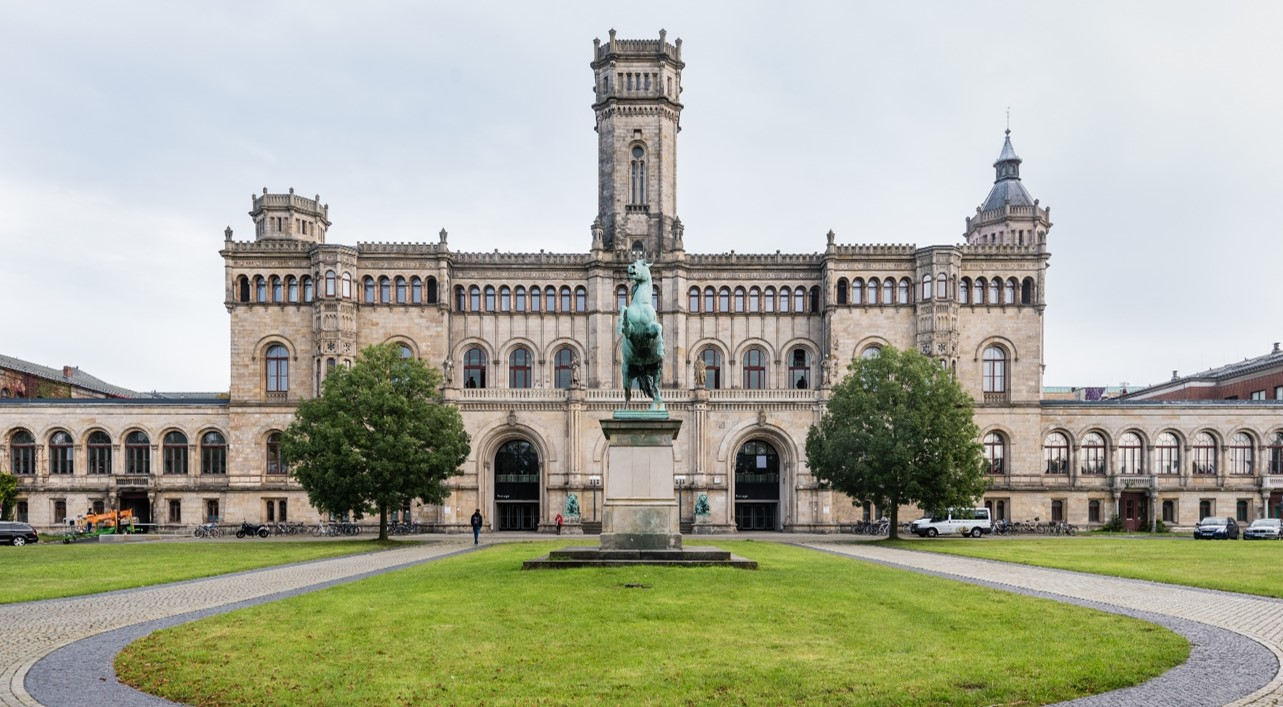
\includegraphics[width=0.65\textwidth]{figures/luh_default_presentation_title_image.jpg}}

% Title page: luhstyle
% \setbeamertemplate{title page}[luhstyle]
% % Add optional title image here
% \addtitlepageimage{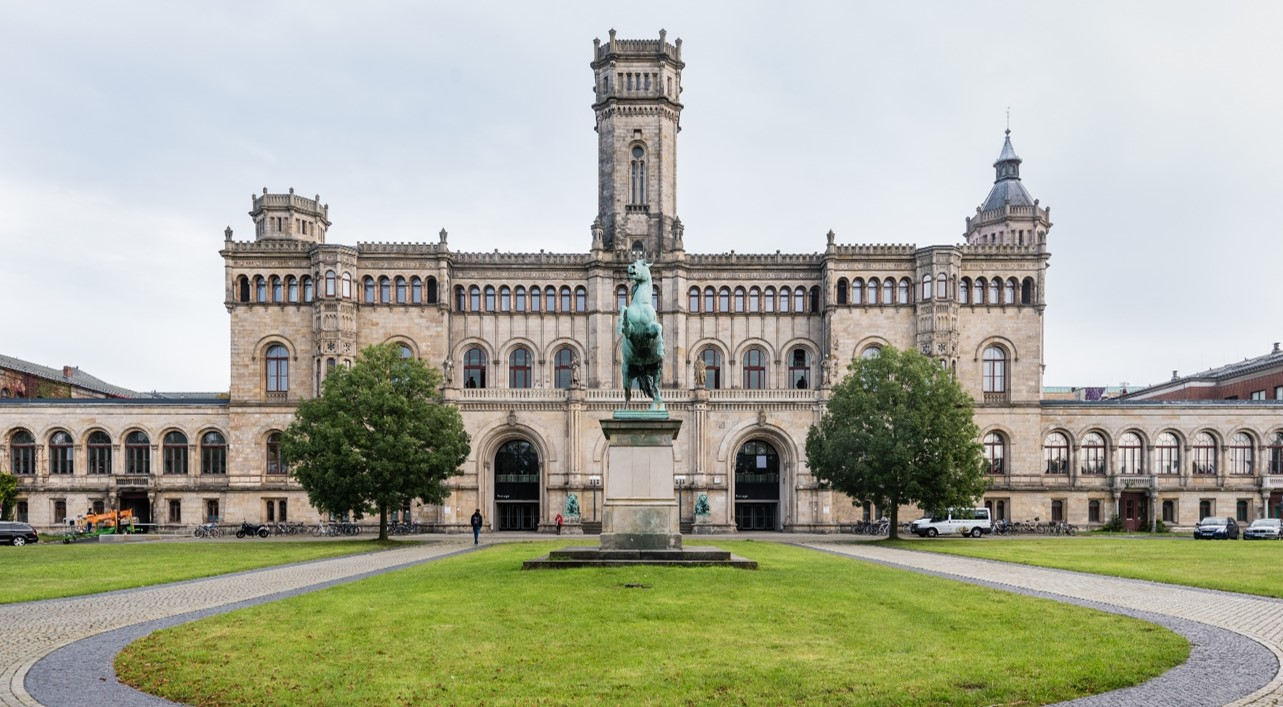
\includegraphics[width=0.75\textwidth]{figures/luh_default_presentation_title_image.jpg}}

\author[Abedjan \& Lindauer]{Ziawasch Abedjan \& Marius Lindauer\\[1em]
	
\includegraphics[height=\logoheight]{../latex_main/figures/luh_logo_rgb_0_80_155.pdf}\qquad
	
\includegraphics[height=\logoheight]{../latex_main/figures/DBIS_Kurzlogo.png}\qquad

\includegraphics[height=\logoheight]{../latex_main/figures/TNT_darkv4}\qquad

\includegraphics[height=\logoheight]{../latex_main/figures/L3S.jpg}	}
\date{Summer Term 2022; \hspace{0.5em} {
\includegraphics[height=1.5em]{../latex_main/figures/Cc-by-nc-sa_icon.svg.png}}; based on \href{https://ds100.org/fa21/}{[DS100]}
}


%%% Custom Packages
%----------------------------------------------------------------------
% Create dummy content
\usepackage{blindtext}

% Adds a frame with the current page layout. Just call \layout inside of a frame.
\usepackage{layout}


%%% Macros
%\renewcommand{\vec}[1]{\mathbf{#1}}
% \usepackage{bm}
%\let\vecb\bm

\title[Introduction]{DS: Bias and Variance}
\subtitle{Bias and Variance in Modeling}

\graphicspath{ {./figure/} }
%\institute{}


\begin{document}
	
	\maketitle
	\begin{frame}{A Constant Model}
	    Let’s say you want to estimate how often a coin lands on heads when flipped.
	    \begin{itemize}
	        \item The result of a coin flip follows a Bernoulli(p) distribution, and you want to estimate p.
	        \item You do not collect any data, but instead you are given a choice between two models.
	        \item Suppose you are also told that p = .5.
	    \end{itemize}
	    Which of the following is the better model?\\
	    \bigskip
	    Model A: Select a random number between 0 and 1. This is your estimate of p. This is equivalent to running np.random.random()in Python.\\
	    \bigskip
	    Model B: Select .75 as your estimate of p.
	\end{frame}
	
	
	\begin{frame}{A Constant Model}
	   How do we define “better”?\\
	   \bigskip
	    We can calculate the expected MSE of each model. This is called the “model risk,” a term which we will formalize later on. The lower the risk, the better.\\
	    \bigskip
	    Model A: On average, we will select .5 as our estimate, so we expect 0 error. But, as we are only selecting one number, there is a chance we select a number really far away from .5.\\
	    \bigskip
	    Model B: With this model, we will never be exactly correct. But, we know there is zero chance of a really terrible prediction.
	\end{frame}
	
	
	\begin{frame}[c]{The Bias-Variance Tradeoff}
	   When building models, we generally face a tradeoff between bias and variance.
	   \begin{itemize}
	       \item Lower bias means that our model will predict closer to the truth, on average.
	       \item Lower variance means that our model will not change too much given the sample.
	   \end{itemize}
	   \bigskip
	   We want low bias and low variance, but oftentimes, when one decreases, the other increases.\\
	   Model A has zero bias, but lots of variance. Model B has zero variance, but lots of bias.\\
	   \bigskip
	   So which is better? The answer will be revealed later in the lecture.
	\end{frame}
	
	
	\begin{frame}[c]{Three Sources of Error in Our Predictions}
	   Irreducible error: Recall the data generating process: $Y = g(x) + \epsilon$
	   \begin{equation*}
	       \mathbb{V}ar(\epsilon) = \sigma^2 \hspace{5mm} \mathbb{V}ar(Y) = \mathbb{V}ar(g(x) + \epsilon) = \mathbb{V}ar(\epsilon) = \sigma^2
	   \end{equation*}
	   There will be chance error in our predictions due to the natural randomness of the world.\\
	   \bigskip
	   Model variance: Our fitted model is based on a random sample.\\
        The sample could have come out differently, then the fitted model would have been different.\\
        \bigskip
        Model bias: This is the difference between the expected predictions, and the true g(x).\\
        Our model may be too limited to find the correct g(x), for example if we pick a quadratic model to fit to cubic data.

	\end{frame}
	
	
	\begin{frame}[c]{Simulation}
	  \begin{columns}
	      \begin{column}{.6\textwidth}
	           \begin{figure}
	               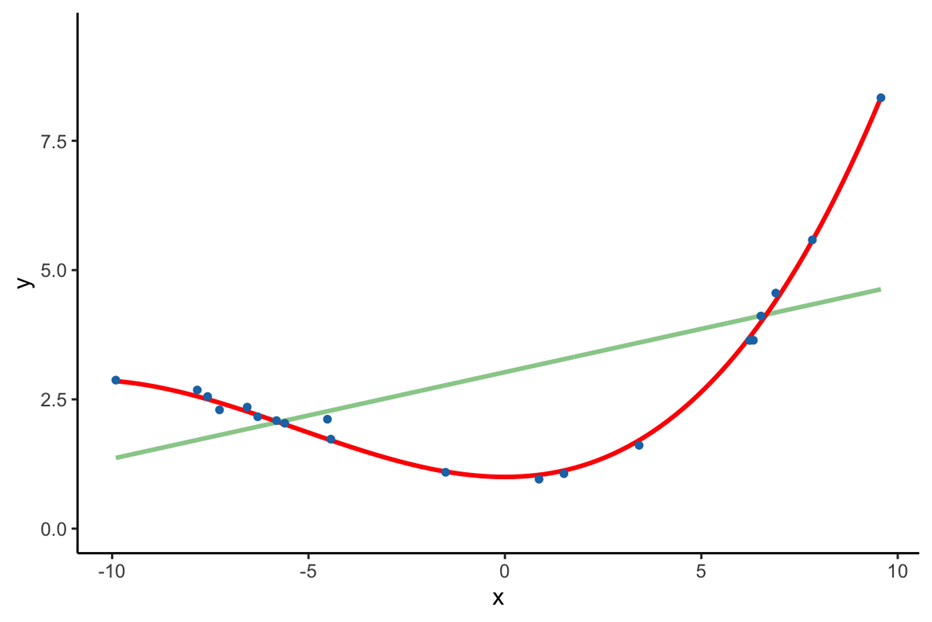
\includegraphics[scale=.5]{Bild9}
	           \end{figure} 
	      \end{column}
	      
	      \begin{column}{.4\textwidth}
	      \\
	      \bigskip
	      \bigskip
	      \bigskip
	            Let’s simulate the sampling and modeling process for a strictly linear model.\\
	            $g(x) = \theta_0 + \theta_1x$
	      \end{column}
	  \end{columns}
	\end{frame}
	
	\begin{frame}[c]{Simulation}
	  \begin{columns}
	      \begin{column}{.6\textwidth}
	           \begin{figure}
	               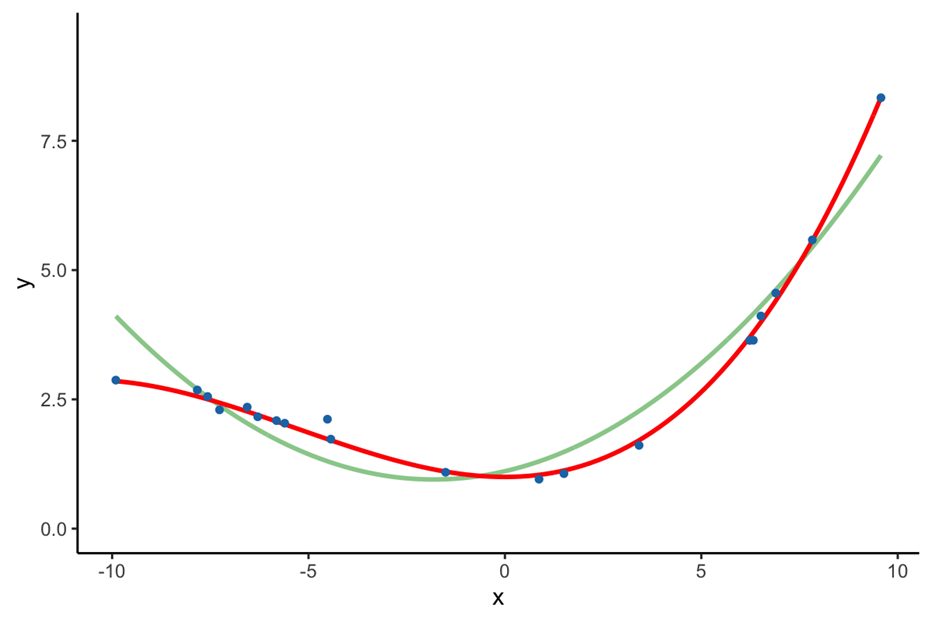
\includegraphics[scale=.5]{Bild10}
	           \end{figure} 
	      \end{column}
	      
	      \begin{column}{.4\textwidth}
	      \\
	      \bigskip
	      \bigskip
	      \bigskip
	            Let’s simulate the sampling and modeling process for a quadratic model.\\
	            $g(x) = \theta_0 + \theta_1x + \theta_2x^2$
	      \end{column}
	  \end{columns}
	\end{frame}
	
	
	\begin{frame}[c]{Simulation}
	  \begin{columns}
	      \begin{column}{.6\textwidth}
	           \begin{figure}
	               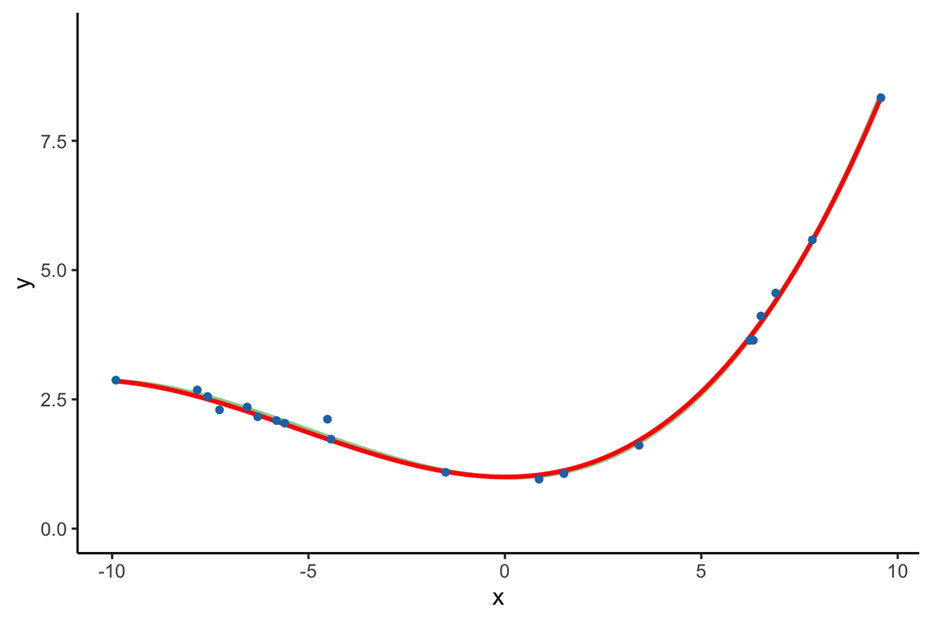
\includegraphics[scale=.5]{Bild11}
	           \end{figure} 
	      \end{column}
	      
	      \begin{column}{.4\textwidth}
	      \\
	      \bigskip
	      \bigskip
	      \bigskip
	            Let’s simulate the sampling and modeling process for a cubic model.\\
	            $g(x) = \theta_0 + \theta_1x + \theta_2x^2 + \theta_3x^3$
	      \end{column}
	  \end{columns}
	\end{frame}
	
	
	
	\begin{frame}[c]{Simulation}
	  \begin{columns}
	      \begin{column}{.6\textwidth}
	           \begin{figure}
	               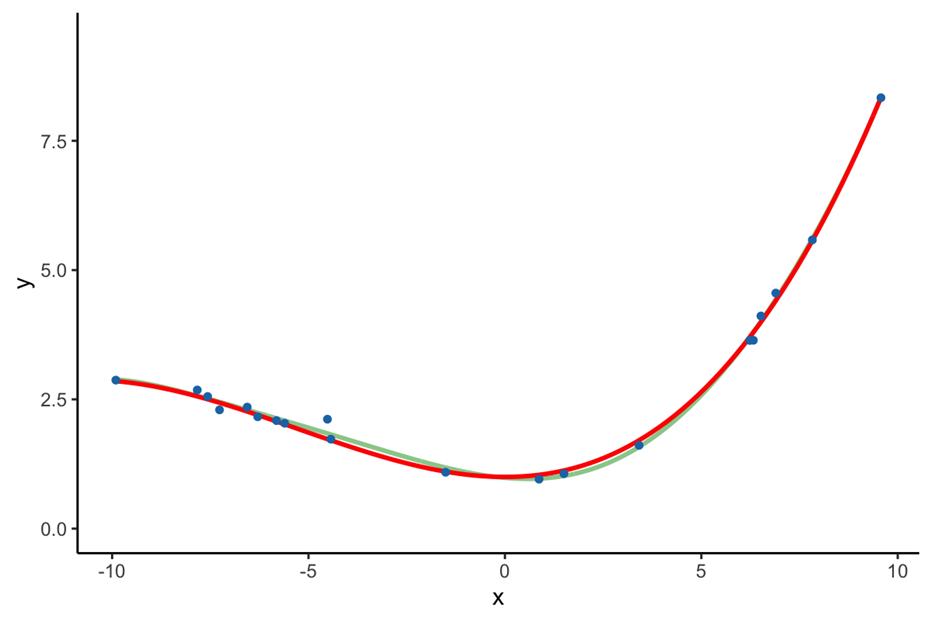
\includegraphics[scale=.5]{Bild12}
	           \end{figure} 
	      \end{column}
	      
	      \begin{column}{.4\textwidth}
	      \\
	      \bigskip
	      \bigskip
	      \bigskip
	           Let’s simulate the sampling and modeling process for a septic model.\\
	            $g(x) = \theta_0 + \sum\limits_{i=1}^7 \theta_ix^i$
	      \end{column}
	  \end{columns}
	\end{frame}
	
	\begin{frame}[c]{Diagram}
	  \begin{columns}
	     
	      
	      \begin{column}{.4\textwidth}
	      \\
	      \bigskip
	      \bigskip
	      \bigskip
	          Red line (fixed): g(X)\\
	          Green line $\mathbb{E}(\hat{Y}(x))$
	          \begin{itemize}
	              \item This is fixed, given our model.
	          \end{itemize}
	          Gray lines: Possible $\hat{Y}(x)$\\
	          Blue points: Y = g(x) + $\epsilon$
	      \end{column}
	      
	      
	       \begin{column}{.6\textwidth}
	           \begin{figure}
	               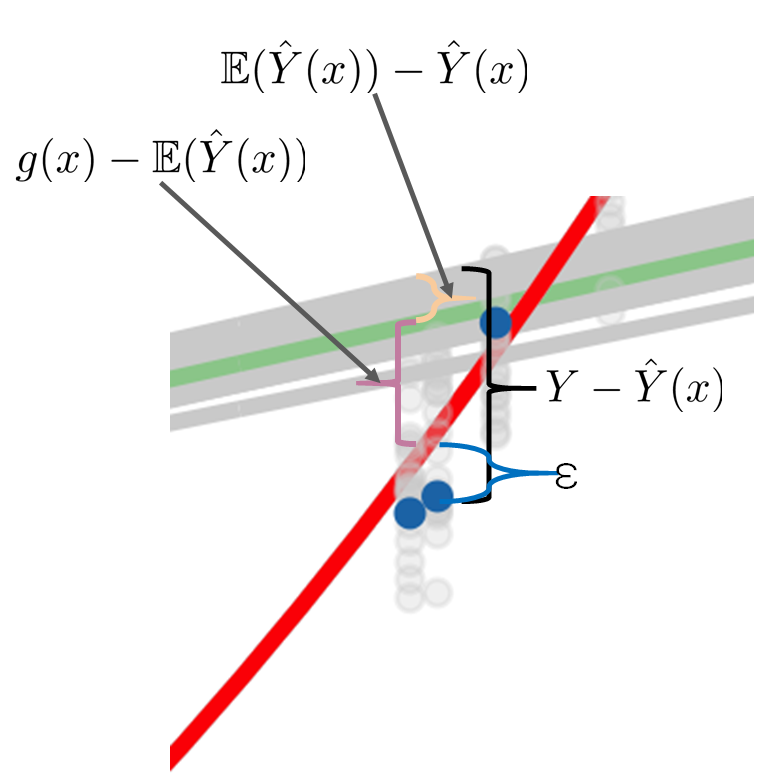
\includegraphics[scale=.3]{Bild13}
	           \end{figure} 
	      \end{column}
	  \end{columns}
	\end{frame}
\end{document}